%% all subsystems insame format
The UR20 arm is the physical UR20 module. It can be controlled the a '3PE Teach Pendant' that allows touchscreen controls, or the Cobot URScript/Python URX library. This module covers the physical arm itself, the control mechanisms, and the gripper used for manipulating boxes.

\subsection{Layer Hardware}
The UR20 arm covers the UR20 arm, the control tablet, the control box, and gripper.

\subsection{Layer Operating System}
The Operating system used will be the UR PolycScope system that runs as the UR robots OS and programming interface.

\begin{figure}[h!]
	\centering
 	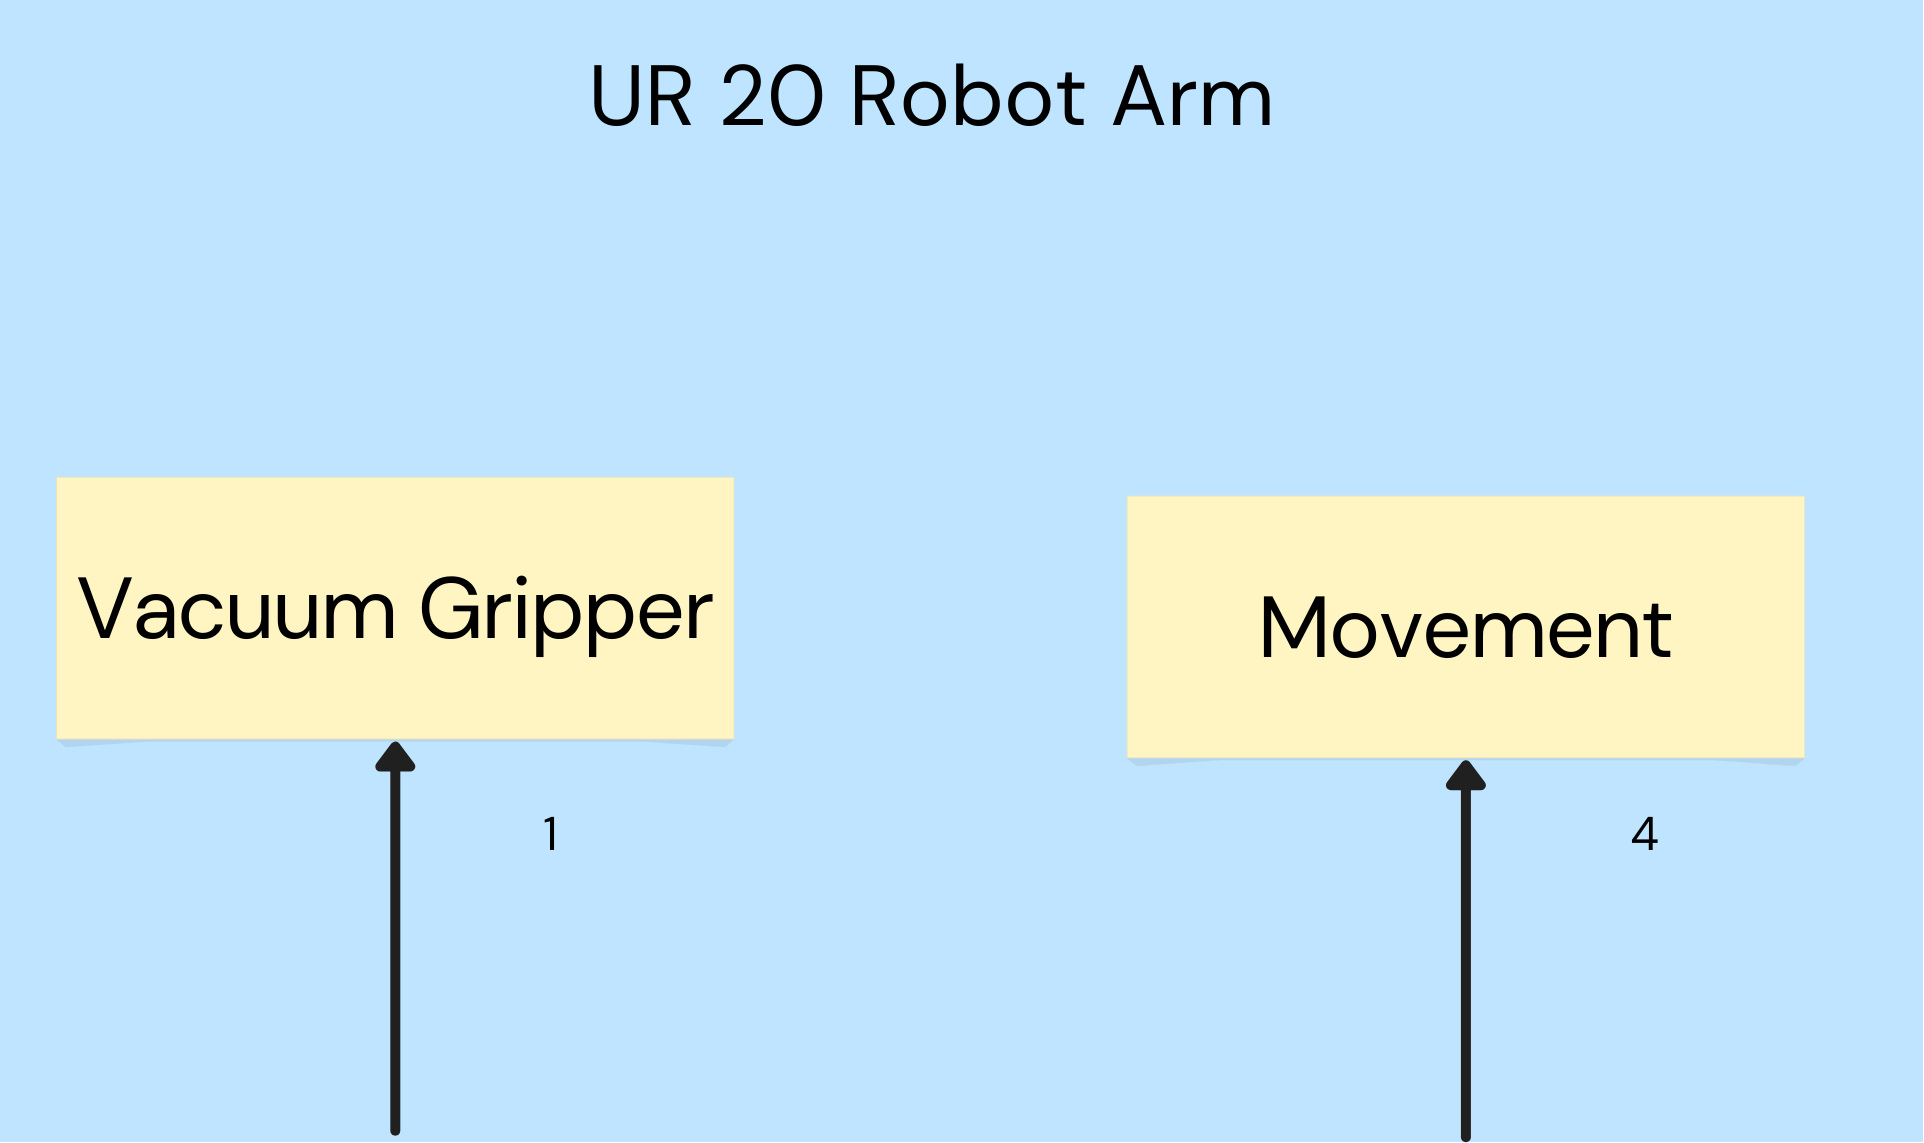
\includegraphics[width=0.60\textwidth]{images/arm}
 \caption{UR20 Arm subsystem}
\end{figure}

\subsection{Vacuum Gripper}
The Vacuum Gripper is tasked with the carrying the the incoming packages from the conveyor belt onto and releasing the package at the appropriate location on the pallet.

\subsubsection{Gripper Software Dependencies}
The Gripper will be dependent on the the voltage assignment of port (TBA) from the PLC to release and hold suction. Controlled through URScript/Python (URX library)

\subsubsection{Vacuum Hardware}
The hardware used in the gripper is the gripper itself as well as the vacuum. The gripper includes the use of an aluminum base plate, suction cups and air tube systems that connects to the vacuum. The vacuum will connect to a control box port for control.

\subsubsection{Vacuum Programming Languages}
The way to control the UR20 gripper will come from the URScript/Python

\subsection{Arm Movement}
The movement subsection of the Layer is input of the current arm location and movement of the arm to is next position whether to be in position place a box in its appropriate position or to return to the conveyor belt and await its next package.

\subsubsection{Arm Hardware}
As for the the hardware it would be the connection of the arm to its control box and control tablet access location and adjust arm position. 

\subsubsection{Arm Programming Languages}
The way to control the UR20 gripper will come from the URScript/Python
